\newpage
МРНТИ 06.75.03

\sectionwithauthors{A.Serikkyzy, S.S. Baktymbet, M. Ermirzoev, A.B. Akhmetova}{THE IMPACT OF FOREIGN AID ON THE ECONOMIC GROWTH OF CENTRAL ASIAN COUNTRIES}

\begin{center}
(analytical review)

{\bfseries \textsuperscript{1}A.Serikkyzy, \textsuperscript{3}S.S.
Baktymbet\textsuperscript{🖂}, \textsuperscript{2}M. Ermirzoev,
\textsuperscript{1}A.B. Akhmetova}

\textsuperscript{1}ALMAU, Almaty, Kazakhstan,

\textsuperscript{2}University of Central Asia, Khorog, Republic of
Tajikistan,

\textsuperscript{3}Academy of Political Management, Astana, Kazakhstan
\end{center}

{\bfseries \textsuperscript{🖂}}Corresponding author: saule\_sbs@mail.ru

This study explores the relationship between foreign financial aid and
economic growth in Central Asian countries. Foreign aid is viewed as a
critical resource for promoting long-term growth by addressing key
challenges such as infrastructure, healthcare, and education. However,
the effectiveness of aid remains contentious, with critics arguing that
it may foster dependency, corruption, and inefficient use of resources.
Central Asia, comprising countries like Kazakhstan, Kyrgyzstan,
Uzbekistan, Tajikistan, and Turkmenistan, has received substantial
foreign financial aid since gaining independence following the
dissolution of the Soviet Union. While some scholars suggest that
foreign aid has positively impacted the economic growth of Central Asian
nations, others argue that it has had minimal or even negative effects.
This study emphasizes the importance of evaluating not only the amount
of aid but also its effectiveness, with a particular focus on the role
of institutional quality in determining the success of aid in promoting
sustainable economic development.

{\bfseries Key words:} foreign aid, economic growth, Central Asia,
dependence, corruption.

\sectionheading{ВЛИЯНИЕ ИННОСТРАННЫХ ИНВЕСТИЦИЙ НА ЭКОНОМИЧЕСКИЙ РОСТ СТРАН
ЦЕНТРАЛЬНОЙ АЗИИ}

\begin{center}
(аналитический обзор)

{\bfseries \textsuperscript{1}А.Серіккызы,
\textsuperscript{3}С.С.Бақтымбет\textsuperscript{🖂},
\textsuperscript{2}М.Eрмирзоев, \textsuperscript{1}А.Б.Ахметова}

{\bfseries \textsuperscript{1}}Университет ALMAU, Алматы, Казахстан,

{\bfseries \textsuperscript{2}}Университет Центральной Азии, г. Хорог,
Республика Таджикистан,

{\bfseries \textsuperscript{3}}Академия политического менеджмента, Астана,
Казахстан,

e-mail:saule\_sbs@mail.ru
\end{center}

В этом исследовании изучается взаимосвязь между иностранными
инвестициями и экономическим ростом стран Центральной Азии. Иностранные
инвестиций со стороны зарубежных государств рассматривается как
критически важный ресурс для содействия долгосрочному росту путем
решения таких ключевых задач, как инфраструктура, здравоохранение и
образование. Однако эффективность помощи остается спорной, поскольку
критики утверждают, что она может способствовать зависимости, коррупции
и неэффективному использованию средств. Центральная Азия, включающая в
себя такие страны, как Казахстан, Кыргызстан, Узбекистан, Таджикистан и
Туркменистан, получила значительную зарубежную финансовую помощь с
момента обретения независимости после распада Советского Союза. В этом
исследовании подчеркивается важность оценки не только количества помощи,
но и ее эффективности, с особым акцентом на роль институционального
качества в определении успеха помощи в содействии устойчивому
экономическому развитию.

{\bfseries Ключевые слова}: иностранные инвестиций, экономический рост,
Центральная Азия, зависимость, коррупция.

\sectionheading{ШЕТЕЛДІК ИНВЕСТИЦИЯЛАРДЫҢ ОРТАЛЫҚ АЗИЯ ЕЛДЕРІНІҢ ЭКОНОМИКАЛЫҚ ӨСУІНЕ ӘСЕРІ}

\begin{center}
(аналитикалық шолу)

{\bfseries \textsuperscript{1}А.Серікқызы, \textsuperscript{3}С.С.
Бақтымбет\textsuperscript{🖂}, \textsuperscript{2}М.Ермирзоев,}
{\bfseries \textsuperscript{1}А.Б. Ахметова}

\textsuperscript{1}Алматы менеджмент университеті ALMAU, Алматы,
Қазақстан,

\textsuperscript{2}Орталық Азия Университеті, Хорог, Тәжікстан
Республикасы,

\textsuperscript{3}Саяси менеджмент Академиясы, Астана, Қазақстан,

e-mail:saule\_sbs@mail.ru
\end{center}

Бұл зерттеу шетелдік қаржылық көмек пен Орталық Азия елдерінің
экономикалық өсуі арасындағы байланысты зерттейді. Шет мемлекеттердің
қаржылық көмегі инфрақұрылым, денсаулық сақтау және білім беру сияқты
негізгі міндеттерді шешу арқылы ұзақ мерзімді өсуге ықпал ететін маңызды
ресурс ретінде қарастырылады. Алайда, көмектің тиімділігі даулы болып
қала береді, өйткені сыншылар бұл тәуелділікке, сыбайлас жемқорлыққа
және қаражатты тиімсіз пайдалануға ықпал етуі мүмкін деп санайды.
Қазақстан, Қырғызстан, Өзбекстан, Тәжікстан және Түрікменстан сияқты
елдерді қамтитын Орталық Азия Кеңес Одағы ыдырағаннан кейін тәуелсіздік
алған сәттен бастап айтарлықтай шетелдік қаржылық көмек алды. Кейбір
ғалымдар шетелдік көмек Орталық Азия елдерінің экономикасының өсуіне оң
әсер етті деп болжаса, басқалары оның шамалы немесе тіпті теріс әсер
еткенін айтады. Бұл зерттеу көмектің мөлшерін ғана емес, оның
тиімділігін бағалаудың маңыздылығына баса назар аударады, бұл тұрақты
экономикалық дамуға көмектесудің сәттілігін анықтаудағы институционалдық
сапаның рөліне ерекше назар аударады.

{\bfseries Түйін сөздер}: шетелдік көмек, экономикалық өсу, Орталық Азия,
тәуелділік, жемқорлық.

\begin{multicols}{2}
{\bfseries Introduction.} The importance of understanding the relationship
between foreign investment and economic growth lies in shaping
appropriate development policies. Financial assistance is considered a
pivotal resource that adds to investment in the domestic country aimed
at long-term growth. It targets priority areas such as infrastructure,
healthcare, and education, which are essential for achieving sustainable
economic growth. At the same time, foreign aid can ensure stability and
act as a catalyst for implementing economic reforms during difficult
times. Despite this, the issue of the effectiveness of foreign aid in
promoting economic growth is widely debated; some authors who are
against foreign aid propose the statement that it can create dependence
and stimulate corruption. At the same time, it is possible that aid will
not be used for the intended purpose and will not directly support
economic policy due to the weak institutional quality. This study
examines foreign aid and economic growth in Central Asia.~

The Central Asian area is primarily comprised of five nations:
Kazakhstan, Kyrgyzstan, Uzbekistan, Tajikistan, and Turkmenistan. These
nations, which were republics of the Soviet Union, underwent significant
changes following the USSR's dissolution in 1991. Throughout this
period, they transitioned from a centrally planned economy to a
market-based economy. Although the transition process provided new
opportunities for growth and development, it caused these states to face
numerous obstacles and challenges.

Eventually, after gaining independence, the Central Asian states started
to receive a substantial amount of foreign aid. Most foreign assistance
came from donors, international organizations such as the World Bank,
International Monetary Fund, European Union, and developed nations,
including the United States, Japan, Germany, and other countries
contributing financially. The funds were intended to reduce the poverty
rate and achieve sustained growth.

Assessing the impact of international financial support on Central Asia
is important, yet this topic remains under debate. Some scholars believe
that foreign aid has a positive effect on growth, while other authors
claim that it does not have any effect or even negatively impacts the
economy. Proponents of aid state that it is essential for growth.
However, opponents of aid argue that it promotes reliance on foreign
funds and contributes to poor governance system or corruption when funds
are wasted. It is essential to analyze the impact of foreign monetary
assistance on economic expansion. Hence, it is important to analyze not
solely the amount of money received but also the efficiency of aid and
growth. Moreover, institutional quality is important because according
to the conventional wisdom higher institutional quality is associated
with the higher effectiveness of aid.

{\bfseries Definition of Aid.} It's worthwhile to mention that aid
encompasses different kinds of resources, such as tangible goods,
concessional loans, and nonrepayable financial grants. The Development
Assistance Committee (DAC) of the Organization for Economic Cooperation
and Development (OECD) represents the largest provider of aid,
consisting of 32 countries. The DAC defines aid as official development
assistance (ODA), which is primarily governmental aid designed for
developing countries\textquotesingle{} well-being and economic growth.
This organization has established specific criteria for identifying the
aid as ODA. First, it should come from the donor
country\textquotesingle s government agencies. The second criterion is
that it should achieve economic growth and contain a 25\% grant element
or more. Every three years, DAC updates its list of ODA receipts based
on the country\textquotesingle s per capita income. The DAC countries
expect recipient republics allocate development aid properly to mitigate
some of the economic challenges. Military aid and increased donor
security do not qualify as ODA. In some cases, aid for developing
countries can be in the form of humanitarian assistance, which includes
food and technical support such as projects or programs (OECD). For this
thesis, foreign aid specifically refers to the ODA.
\end{multicols}

\begin{figure}[H]
	\centering
	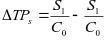
\includegraphics[width=0.7\textwidth]{assets/341}
	\caption*{Figure 1 - Total ODA for Central Asia, 2000-2020 {[}1{]}.}
\end{figure}

\begin{multicols}{2}
{\bfseries Overview of Aid in Central Asia}{\bfseries .} As previously
mentioned, Central Asian countries began to receive foreign aid after
the collapse of the USSR. However, the countries did not receive the
same level of aid, and its distribution varied among them both in terms
of the amount received and the type of aid. For some developed
countries, providing foreign aid was a means of strengthening their
involvement in the region. Foreign aid from donor countries to Central
Asia mainly had a positive impact on the humanitarian, economic, and
social sectors of the economy. The DAC members directed most of the
foreign aid to the region. Notable China is not listed among these DAC
members, although it has been and continues to be one of the main
creditors for some Central Asian countries. Foreign aid, commonly
referred to as ODA (Official Development Assistance), primarily involves
the repayment of loans on concessional terms, such as the net repayment
of the principal and grant element, which includes at least 25\%,
estimated at a 10\% discount rate (OECD, 2024). From 2000 to 2020,
Central Asia received a total of \$11.57 billion in ODA from various
bilateral donors. Figure 1 below shows the distribution of ODA
throughout the region for the period 2000--2020.

From figure 1, in 2011, Central Asia received the least amount of the
ODA, totalling \$412.38 million, and in 2019, the region received the
highest amount, \$931.28 million. Figure 2 displays the amount of ODA
receipts from 2000 to 2020.
\end{multicols}

\begin{figure}[H]
	\centering
	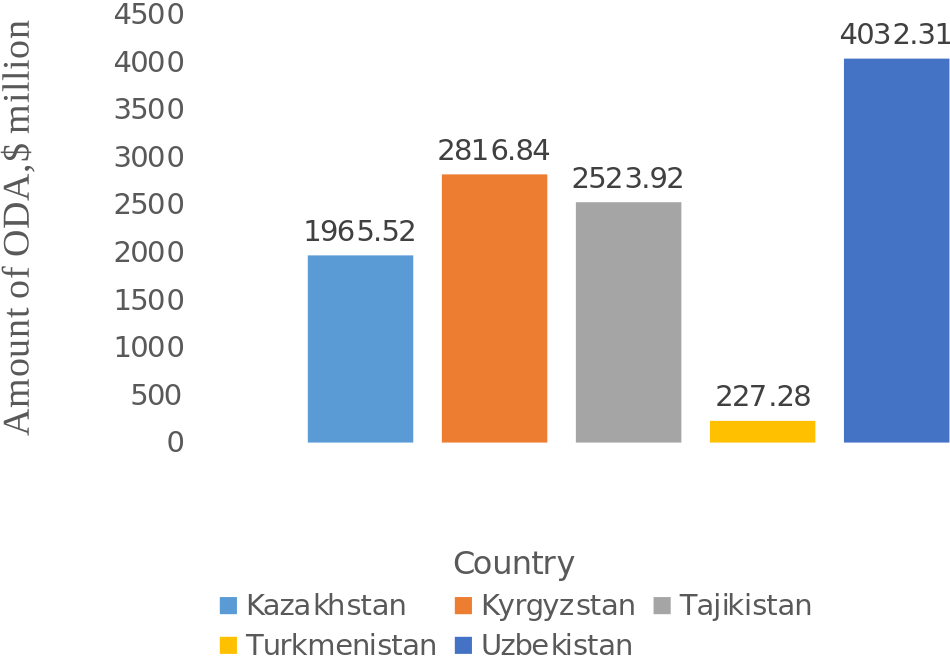
\includegraphics[width=0.7\textwidth]{assets/341.1}
	\caption*{Figure 2 - Net ODA classification by country {[}1{]}}
\end{figure}

\begin{multicols}{2}
Uzbekistan leads in ODA receipts between 2000 and 2020, totaling \$4.3
billion. Following closely, Kyrgyzstan secures the second-highest amount
with \$2.82 billion. Notably, Kyrgyzstan was the first among Central
Asian countries to implement IMF policies. Tajikistan follows in third
place, having received \$2.52 billion. Uzbekistan takes the fourth spot,
with a net official ODA receipt of \$1.97 billion. Finally, Turkmenistan
concludes the list among Central Asian recipients, having received
\$227.8 million during the specified period.

{\bfseries Country Specific Trends}. Even though Central Asian countries
received different amounts of ODA from bilateral and multilateral
organizations throughout the period of 2000--2020, most of these states
had the same major donor. Next, the following subsection will describe
the ODA distribution for every Central Asian entity. It will mention the
prominent donors, the total amount of aid received, and the impact of
such aid on socioeconomic development.

{\bfseries Aid in Kazakhstan.}
\end{multicols}

\begin{figure}[H]
	\centering
	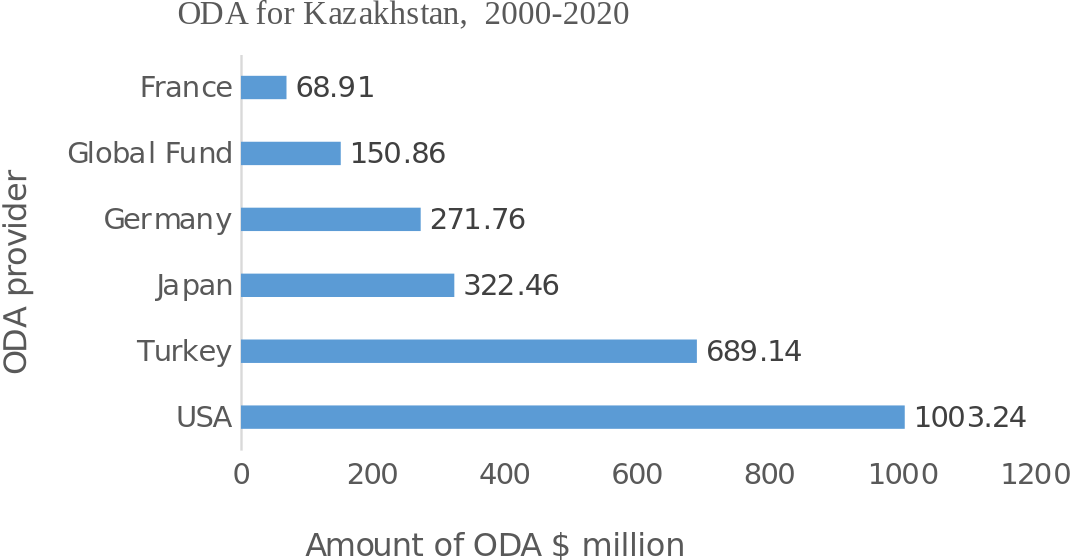
\includegraphics[width=0.7\textwidth]{assets/341.2}
	\caption*{Figure 3 - Main ODA providers for Kazakhstan, 2000-2020 {[}1{]}}
\end{figure}

\begin{multicols}{2}
The USA is the largest ODA provider for Kazakhstan, offering \$1 billion
from 2000--2020. Like other donor countries, the USA targets specific
areas within Kazakhstan for its funds, including the social sector,
judiciary, and civil society. Additionally, it supports trade
opportunities and aids in the development of low-cost energy. Among
Central Asian countries, Kazakhstan allocates a sufficient budget to its
energy sector, with the US Agency for International Development (USAID)
actively supporting and promoting green energy policies {[}2{]}.

From 2000 to 2020, Kazakhstan received the highest amount of Official
Development Assistance (ODA) from Turkey. The Turkish Cooperation and
Coordination Agency's (TIKA) is an important aid provider focusing on
agricultural and livestock areas. In addition, TIKA supports the
improvement of social life standards through employment and vocational
training programs. Also, the agency supports the conservation of the
same historical and cultural identities {[}3{]}. This organization in
Kazakhstan also aims to improve the road infrastructure.

In 1997, Japan started to come up with Eurasian diplomacy, establishing
a political corporation with Kazakhstan and subsequently providing
investment in the energy sector. One of the highlighted projects between
Kazakhstan and Japan was the Silk Road Energy Mission. The "Central Asia
plus Japan" dialogue guided the project\textquotesingle s operation. The
aim of this project, accepted in 2006, was to enhance and promote atomic
energy safety and nuclear security. In essence, these two countries
share mutual benefits, particularly in the field of nuclear energy.
While Japan possesses advanced technology, it lacks some of its natural
resources, leading it to seek a high supply of uranium for its growing
nuclear energy sector. Kazakhstan, with the second-largest uranium
reserves, provides Japan with this resource. Cooperation agreements
between these countries primarily include investments in the nuclear
power industries, uranium mines, and technology exchange {[}4{]}.

Germany is the third country to strongly support Kazakhstan. During the
specified period, this country provided Kazakhstan with \$271.76
million. The GIZ organization directed the aid. Germany wants to
allocate its Official Development Assistance (ODA) to Kazakhstan for
education and sustainable economic development. This country, like the
United States, also allocates its ODA for training and employment
purposes. Additionally, Germany is concerned regarding environmental
challenges, public safety, and disaster prevention {[}5{]}.~

{\bfseries Aid in the Kyrgyz Republic.} Among Central Asian countries,
Kyrgyzstan was the first to adapt the IMF policies, which contributed to
receiving significant ODA since its independence. Countries like Japan,
Turkey, Germany, Switzerland, and international organizations like the
Asian Development Bank (Japan), the International Development
Assassination (IDA), and the United Nations (UN) are the main aid
providers for the Kyrgyz Republic. Figure 4 shows the main ODA providers
in Kyrgyzstan from 2000--2020.
\end{multicols}

\begin{figure}[H]
	\centering
	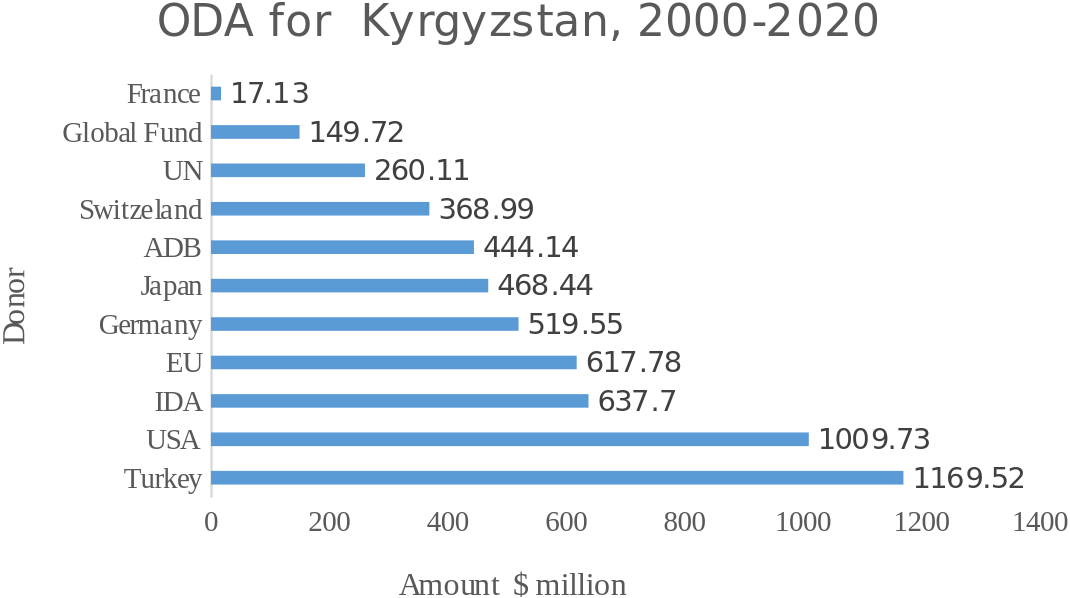
\includegraphics[width=0.7\textwidth]{assets/341.3}
	\caption*{Figure 4- Main providers of ODA for Kyrgyzstan, 2000-2020
{[}1{]}}
\end{figure}

\begin{multicols}{2}
Although Russia is not included in the chart as the country was not
listed in the OECD database, it's noteworthy that the Russia began
providing financial assistance to Kyrgyzstan once they became part of
the Eurasian Economic Union (EEU). In 2015, Russia and the Kyrgyzstan
established a development fund containing \$1 billion. The main aim of
the Russia-Kyrgyz fund was to enhance the economic corporation between
these countries and modernize the Kyrgyz economy. According to the
Development aid report (2018) out of the \$1 billion, \$5000 million
were allocated from the Russian Federal Bank to the National Bank of
Kyrgyzstan. It should be mentioned that these ODA from the Russian fund
was not given for free; Kyrgyzstan will need to repay the loan later.
Top of Form.

Between 2000-2020, Turkey provided the Kyrgyzstan a total \$1169.52
million. The Turkish Cooperation and Coordination Agency (TIKA)
contributed significant amount of foreign aid to Kyrgyzstan, funding
over 760 distinct projects. TIKA wants its money in Kyrgyzstan to be
allocated for the education, infrastructure, and some portion for the
humanitarian purposes {[}6{]}.

USAID is considered one of the largest ODA providers for Kyrgyzstan.
During the mentioned period, the United States allocated \$1009.73
million to Kyrgyzstan. USAID primarily focuses on improving the
governance of the country. Additionally, the USA aims to develop and
promote the business environment and agriculture. Besides these
priorities, the USA also endeavours to positively contribute to various
sectors of the country, including education, healthcare, and human
rights {[}7{]}.

USAID is considered one of the largest ODA providers for Kyrgyzstan.
During the mentioned period, the United States allocated to the
Kyrgyzstan \$1.01 billion. USAID primarily focuses on improving the
governance of the country. Additionally, it promotes the business
environment and agriculture. In addition, the USA endeavors to make
positive contributions to various sectors, including human rights,
education, and healthcare {[}7{]}.

The Asian Development Bank (ADB) is a major multilateral organization
providing funds for Kyrgyzstan development. Between 2000 and 2020, it
allocated a total of \$444.14 million. Mainly ADB's support primarily
focuses on road's rehabilitation projects like Bishkek-Osh and the
Bishkek -Torugart routes, which connects the country's north and south
and link it with China {[}6{]}. Beside the road improvement in
Kyrgyzstan, ADB invests in various sectors such as education,
governmental structures, and the civil society. It also plays a
significant role in promoting water supply initiatives to facilitate
hydropower expansion. Notably, ADB undertook the rehabilitation of
Kyrgyzstan largest and most important power station of this country as
part of its project {[}7{]}.

Alongside with other international ODA providers, IDA stands out as a
major donor for Kyrgyzstan. From the period of 2000-2020 this
organization provided \$637.7 million in comprising both loans and
grants. IDA allocates its ODA towards the energy, agriculture, and
transportation initiatives {[}7{]}.

{\bfseries Aid in Tajikistan}. Like other Central Asian countries,
Tajikistan has also started to receive a significant amount of ODA since
its independence. Figure 5 illustrates the primary ODA allocation for
this country.
\end{multicols}

\begin{figure}[H]
	\centering
	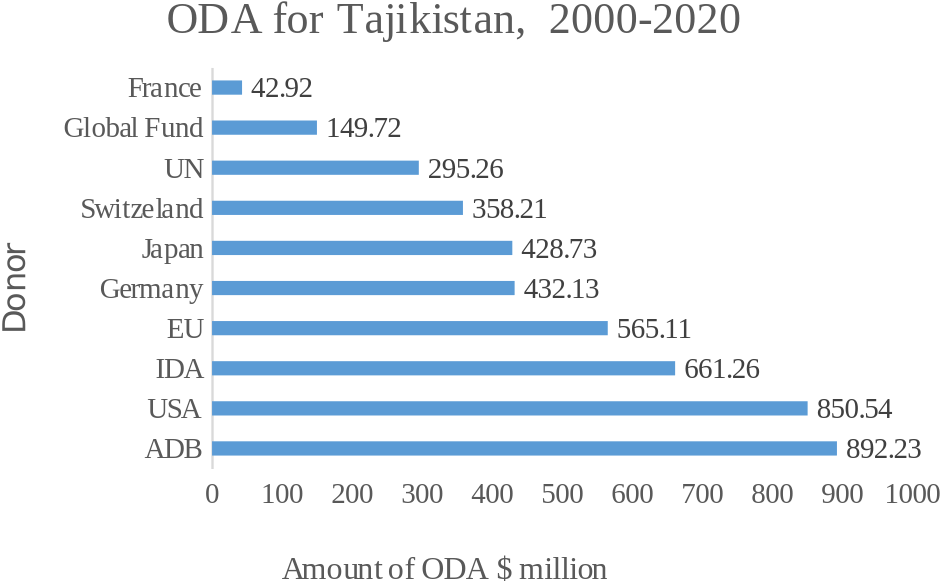
\includegraphics[width=0.7\textwidth]{assets/341.4}
	\caption*{Figure 5 - Main ODA providers Tajikistan 2000-2020 {[}1{]}}
\end{figure}

\begin{multicols}{2}
From Figure 5, it's evident that ADB was Tajikistan\textquotesingle s
primary ODA provider between 2000 and 2020, contributing a total of
\$892.23 million. It began its collaboration with Tajikistan in 1998.
Initially, this country used ADB's funds for road construction. From
2005 to 2013, this organization facilitated the implementation of
Dushanbe-Kyrgyz Board Rehabilitation Project Phase 2. The ADB allocated
\$51.7 million for this project to improve and resurface the roads and
enhance the drainage systems, bridges, and walls {[}8{]}. This
organization had a significant and positive impact on the
country\textquotesingle s regional corporations and trade. Moreover, the
ADB projects led to the rehabilitation of three hydropower plants in
Tajikistan. In 2008, it allocated \$54.8 million for the ``Nurek 500
Kilovolt Switchyard Reconstruction Project {[}9{]}. Additionally, the
ADB directed its funds to enhance the country\textquotesingle s business
environment, social protection, tax policy, and finance system, while
also promoting employment through private partnerships, vocational
training, and food security promotion {[}10{]}.

From 2000 to 2020, USAID was Tajikistan\textquotesingle s second-highest
ODA provider. Primarily, USAID focuses on enhancing food security,
nutrition, and education while also aiming to improve institutional
quality. USAID strives to improve institutional quality by enhancing
government accountability, credibility, and oversight of basic services.
Moreover, it provides training and access to information for migrant
workers and civil society members. Additionally, this organization
places high value on human rights and tries to inform Tajikistan's
citizens about their rights {[}11{]}.

Tajikistan joined the International Development Association organization
in 1994, a year before joining the World Bank. The IDA directed its
funds towards mitigating climate risk and addressing natural disasters.
Additionally, this organization assists Tajikistan with electricity
exports and economic diversification {[}12{]}.

The European Union (EU) also aids Tajikistan. Primarily, the EU focuses
on three targets: rural development, education, and health. In
Tajikistan, the EU\textquotesingle s primary goal is to reduce poverty
in remote and rural areas by fostering inclusive economic activities in
agriculture and other sectors, thereby creating wealth and job
opportunities. Furthermore, like other international organizations, the
EU values sustainability and encourages the efficient use of natural
resources, as well as the enhancement of resilience to severe weather
conditions. Thanks to EU aid, Tajikistan greatly benefits, particularly
from projects promoting education, regional trade, and enhancing the
private sector and regional trade {[}13{]}.

{\bfseries Aid in Turkmenistan.} Among the central Asian countries,
Turkmenistan received the least amount of ODA. Figure 6 shows the
primary ODA providers in this country for the period 2000--2020.
\end{multicols}

\begin{figure}[H]
	\centering
	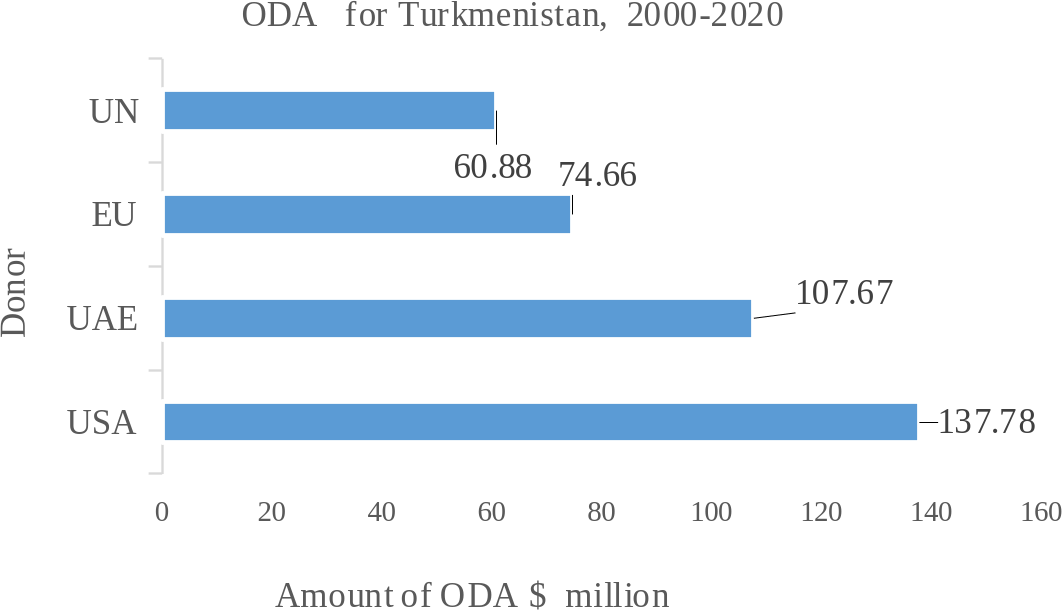
\includegraphics[width=0.7\textwidth]{assets/341.5}
	\caption*{Figure 6 - Main ODA providers for Turkmenistan, 2000-2020
{[}1{]}}
\end{figure}

\begin{multicols}{2}
USAID is one of the largest ODA providers for Turkmenistan, with a total
of \$137.78 million. Like other Central Asian states, this organization
focuses on developing the health sector and youth initiatives in
Turkmenistan. Moreover, USAID assists local entrepreneurs by creating
different job opportunities and enhancing their competitiveness to
increase revenue. To foster citizens' trust in governmental
organizations, USAID promotes and encourages the use of e-governance
technologies, which positively impact information awareness and service
delivery {[}14{]}.

Another large donor for Turkmenistan is the United Arab Emirates (UAE),
which granted \$107.67 million. This country is one of Turkmenistan's
largest business partners, focusing on development corporations.
Infrastructure and road construction are areas of particular interest
for both states, including UAE and Turkmenistan. Additionally, they
prioritize areas such as science, education, culture, and heritage as
crucial components for developing and strengthening their relationship.

In total, the European Union provided \$74.66 million to Turkmenistan
from 2000 to 2020. This organization prioritizes its funds for
expenditure on public administrations and finances. Additionally, the EU
supports the country's private sector and agriculture, especially in
rural and remote areas. Moreover, this organization focuses on improving
the education system, addressing water and environmental problems, and
enhancing law enforcement. Finally, the EU endeavours to mitigate
political issues such as border management and assists in the training
of border guards {[}15{]}.

The United Nations Development Program (UNDP) operates prominently in
Turkmenistan, concentrating on achieving economic prosperity. Primarily,
this organization collaborates with partners to address social issues
such as human development, environmental sustainability, and energy
{[}16{]}.

{\bfseries Aid in Uzbekistan.}
\end{multicols}

\begin{figure}[H]
	\centering
	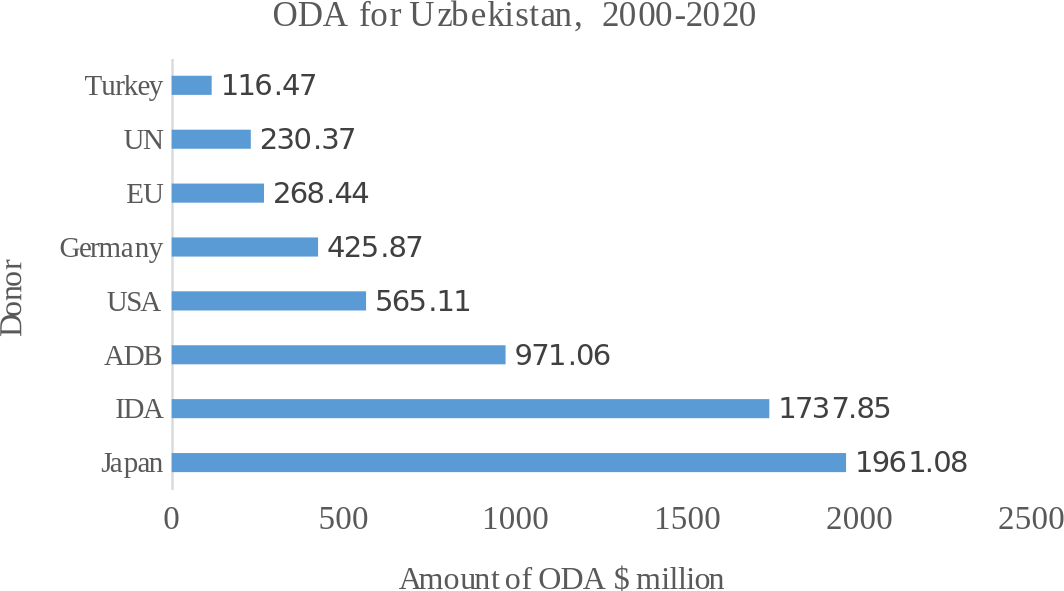
\includegraphics[width=0.7\textwidth]{assets/341.6}
	\caption*{Figure 7- Main ODA providers for Uzbekistan, 2000-2020 {[}1{]}}
\end{figure}

\begin{multicols}{2}
Japan emerges as the largest aid provider for Uzbekistan for the period
of 2000-2020. Japan International Cooperation Agency (JICA) executes a
variety kind of initiatives including grants, concessional loans, and
the technical assistance. This organization allocates ODA towards
railroad projects, power generation, healthcare, agriculture, and other
sectors. A notable JICA program in Uzbekistan is the "Country Assistance
Policy to Uzbekistan ``established in 2012. It aims to stimulate
economic growth by addressing inequality and improving the economic
infrastructure {[}17{]}. Top of Form

In total Uzbekistan received \$1.74 billion from IDA, an agency under
the World Bank. The main aim of the provided ODA from the World Bank was
intended reducing poverty, achieving sustainable economic development,
improving the energy sector, and advancing market reforms. Overall, 28
projects of the World Bank are being implemented in Uzbekistan aiming to
rehabilitate irrigation and drainage system, improve the utility
infrastructure while fostering the economic growth of the country
{[}18{]}.

For the period of the 2000-2020 ADB provided to the Uzbekistan total
amount of the ODA \$7.6 million. Some part of this fund was directed
towards the development particularly for the electricity generation
projects. Under the Central Asian Regional Economic Cooperation (CAREC)
project, ADB in Uzbekistan supports road and railroad projects.
Additionally, ADB aided in providing access to clean water supply for
over 3 million people. Through the "Water Supply and Sanitation Services
Investment Program," more than 4,800 new households gained access to
clean water, and over 170,000 people were provided with improved sewage
services. ADB also assisted the agricultural sector, benefiting over 3.2
million individuals with water provision for agriculture and promoting
crop variety expansion and private sector engagement in horticultural
supply chains.Top of Form

Central Asian countries have benefited from the donor activities from
both DAC countries and international organizations. Major donors for
this region include Turkey, Japan, USA, and Germany while multilateral
organization such as ADB, USAID, IDA, and the EU also play a significant
role. The aim of DAC countries' assistance is mainly directed towards
the improvement of democracy and governance institutions. In Uzbekistan
and Kazakhstan, the focus of most aid is on improving the energy sector
while in Tajikistan and Turkmenistan a major portion of ODA is directed
towards transportation and the storage sector.

{\bfseries The Role of Specific ODA Providers to Central Asia}. Russia and
China are considered major~actors of the~``Eurasian''~and~``Shanghai
spirits''~for the economic development in Central Asia. These countries
are not part of the OECD, still these countries provide a significant
amount of ODA to the region.

{\bfseries Chinese Aid to Central Asia.} Even though China is not a part of
the DAC ODA providers, still it provides enough money to the Central
Asia through the programs like Belt and Road Initiative; It is worth
mentioning that China has a different definition and categorization of
the aid, which is broader than the one outlined by OECD. For example,
for China FDI, commercial loans are also considered as parts of the
foreign aid. Chinese aid is complex, and its statistics is released
through the governmental agencies. This country government set certain
rules based on which it provides it financial assistance to the rest of
the world. The following are eight principles based on which this
Chinese aid should be operated {[}19{]}.

\begin{enumerate}
\def\labelenumi{\arabic{enumi}.}
\item
  The aid provided by the Chinese government is based on the mutual
  benefits it has to the donor and the recipient. It is presented as a
  mutual exchange rather one-side charity.
\item
  The Chinese government does not place any conditions to the recipient
  country as they respect other country rules of law.
\item
  The aid is low-interest or free-interest loans that have the flexible
  repayment period.
\item
  The Chinese aid does not create the dependency but rather enables the
  recipient countries to achieve economic gains.
\item
  The Chinese assistance supports projects that require little spending
  but generate faster profits. This is because the success of such
  projects creates revenue for the recipient country and acquires
  capital.
\item
  The aid includes Chinese domestic machinery and if they fail to meet
  the agreed standard, China can replace them for free.
\item
  The Chinese government also enforces a high level of technical
  assistance to the recipient country and provides the recipient with
  its experts.
\item
  The Chinese experts sent for assistance to the recipient countries are
  expected to work under the same standards as local specialists.
\end{enumerate}

One of the papers devoted to the analysis of Chinese aid and its role in
Central Asia was written by Kashin and Korolev {[}20{]}. The authors of
this article underline the change in the vector of Chinese aid: from
being based on ideological driven agendas during the Cold war to more
economically focused objectives that mainly directed to the interests of
China as a whole.

Kashin and Korolev {[}20{]} also note that the in the past China
provided financial assistance to strengthen the position of Beijing role
in the world and overcome the international isolation. In addition, aid
from China has become one of the main tools to establish contacts with
the other countries.

Kashin and Korolev provide the critical assessment of the Chinese aid.
According to the authors despite the positive effect of Chinese aid to
the region, there might be some strategic motivation behind it. They
mention that even though Chinese aid in Central Asia promotes stability
and development, to some extend it is increasing its power to influence
the region. The authors state that the aid from China to Central Asia is
mostly aimed at infrastructure projects. One such example is the ``Silk
Road Economic Belt''. They argue that such projects not only support the
economic development of the region but also provides opportunity to
China to utilize its industrial capacity.

Authors mention that despite Chinese aid having its positive effects,
still some people believe that it raises concerns regarding becoming
dependent on it. For several years the inflow of Chinese capital to
Central Asia was directed toward infrastructure development which
further boosted the local economies and positively impacted the trade
relationships {[}20{]}.

The frame of China aid to Central Asia is based on the principles of the
mutual benefits of both parties. Mostly, a large amount of Chinese aid
in Central Asia is used for the economic infrastructure mainly the
construction of roads and extractive industries. Up to 2016, China has
granted Central Asia nearly \$30 billion dollars of concessional loans,
most of this amount was allocated to Kazakhstan and Turkmenistan
{[}20{]}.

Another paper about Chinese aid to the Central Asia was published by the
Nargiz Kassenova {[}21{]}. The study emphasizes the significance and
role of China's foreign aid to the region. According to her study
China's development assistance for the region also involves providing
buses, tractors, military supplies, and other kind of the equipment.
Additionally, China provides governmental scholarships to Central Asian
students and training programs for civil workers and military personnel.

Moreover, with both studies by Kassenova and Kashin and Korolev, China's
strategic use of its aid in Central Asia is questioned due to the
diverse objectives behind China's assistance. While Kashin and Korolev
argue that there has been a change to more economic variants from
ideologically driven agendas, they cannot deny the strategic motivation
on China's part. While the second article claims that the country's aid
is used to build strong social ties to the Central Asia. Both studies
explain mention about the goals of China's foreign aid within this
region, showcasing its economic aims in a broader sense.

{\bfseries Russian Aid to Central Asia.} Economically Russia has a dominant
influence in the energy sector, particularly~in countries like
Kazakhstan and Uzbekistan.~Additionally, Russia is interested in
some~sectors~like agriculture, construction, telecommunication, and
mining. Traditionally Russian aid to CA mainly focuses on region's
low-income countries~including~Tajikistan and Kyrgyzstan. In 2010,
Russian bilateral aid to Kyrgyzstan amounted \$25million.
Russia~provides its~aid~through the frameworks~such as the CIS and the
Economic Community.~According to the author~in~recent~years~Russia
forgave a significant amount of~aid~for Kyrgyzstan and Tajikistan for
securing the military cooperation~which~in total amounted~the~\$489
million {[}22{]}.

{\bfseries Conclusion.} Understanding the complex relationship between
foreign aid and economic growth is crucial for shaping effective
development policies, particularly in regions like Central Asia. While
foreign aid has the potential to drive long-term economic development by
addressing critical areas such as infrastructure, healthcare, and
education, its effectiveness remains a subject of debate. In Central
Asia, foreign assistance has played a significant role in the
post-Soviet transition period, with funds aimed at reducing poverty and
promoting sustained growth. However, concerns about aid dependency,
corruption, and inefficient use of funds persist. The impact of foreign
aid ultimately hinges on factors such as institutional quality, which
plays a pivotal role in determining the success of financial support in
fostering economic growth. Thus, a thorough evaluation of both the
quantity and the effectiveness of aid is essential to understanding its
true impact on the economic development of the region.

\emph{{\bfseries Financing}. This work was financially supported by the
Science Committee of the Ministry of Science and Higher Education of the
Republic of Kazakhstan (grant AP1968020, 2023--2025).}
\end{multicols}

\begin{center}
{\bfseries References}
\end{center}

\begin{noparindent}
1.
OECD ODA trends and statistics. -2024. URL:
https://www.oecd.org/en/topics/sub-issues/oda-trends-and-statistics.html
(date of application - 12.09.2024)

2.
Galante, A. How the U.S. benefits from foreign aid to Kazakhstan. The
Borgen Project. -2018. URL:
https://borgenproject.org/us-benefits-foreign-aid-kazakhstan/ (date of
application - 12.09.2024)

3.
Fidan, H., \& Nurdun, R. Turkey's role in the global development
assistance community: the case of TIKA (Turkish International
Cooperation and Development Agency) // Journal of Southern Europe and
the Balkans. -2008. --Vol. 10(1). --P. 93--111.
https://doi.org/10.1080/14613190801895888 (date of application
12.09.2024)

4.
Kassenova, T\& Toki, M. Japan and Kazakhstan: nuclear energy
cooperation. The Nuclear Threat Initiative. -2010. URL:
https://www.nti.org/analysis/articles/japan-kazakhstan-energy-cooperation/
(date of application - 12.09.2022)

5.
German Federal Foreign Office, Germany and Kazakhstan: Bilateral
relations. -2024. URL:

https://www.auswaertiges-amt.de/en/aussenpolitik/laenderinformationen/kasachstan-node/kazakhstan/

218898
(date of application - 12.09.2024)

6.
Gunaydin, H. C. Turkey funded over 760 aid projects in Kyrgyzstan.
Turkey (2018).

7.
Development Aid. Donor activity in the Kyrgyz Republic: Special Report
2018.

https://events.developmentaid.org/attachment/ce1d8bd8-d82a-445a-a907-60db0b82f951/Kyrgyzstan

\%20Report\%202018\%20-\%20Donor\%20Assistance\%20to\%20the\%20Kyrgyz\%20Republic.pdf
Date of application - 12.09.2024

8.
ADB Report Upgraded Tajikistan Road Improves Access to Markets. -2014.
URL:

https://www.adb.org/results/upgraded-tajikistan-road-improves-access-markets

(date of application - 12.09.2024)

9.
ADB Report Tajikistan Hydropower: Strengthening the Power Supply.
-2014.

https://www.adb.org/results/tajikistan-hydropower-strengthening-power-supply

(date of application - 12.09.2024)

10.
ADB Report Tajikistan Farmers Get Affordable Financing to Boost Food
Supply. -2014. URL:

https://www.adb.org/results/tajikistan-farmers-get-affordable-financing-boost-food-supply

(date of application - 12.09.2024)

11.
USAID (n.d). Agriculture and Food Security in Tajikistan. URL:
https://www.usaid.gov/tajikistan/

agriculture-and-food-security (date
of application - 12.09.2024)

12.
World Bank (n.d). Tajikistan - Energy Emergency Recovery Assistance
Project (English). Washington, D.C: World Bank Group.
http://documents.worldbank.org/curated/en/495351468133515937/Tajikistan-Energy-Emergency-Recovery-Assistance-Project
(date of application - 12.09.2024)

13.
European Commission (n.d). Tajikistan. URL:

https://international-partnerships.ec.europa.eu/countries/tajikistan\_en
(date of application - 12.09.2024)

14.
USAID (n.d). USAID Turkmenistan. URL:

https://www.usaid.gov/turkmenistan\#:\textasciitilde:text=In\%20Turkmenistan\%2C\%20USAID\%20advances\%20

the,and\%20respect\%20for\%20human\%20rights\%3B
(date of application - 12.09.2024)

15.
European Union European Union and Turkmenistan. -2021.
https://www.eeas.europa.eu/turkmenistan/

european-union-and-turkmenistan\_en?s=231
(date of application - 12.09.2024)

16.
UNDP UNDP Turkmenistan. -2024. --URL:
https://www.undp.org/turkmenistan (date of application - 12.09.2024)

17.
JICA (n.d). Official Aid from Japan to Uzbekistan. URL:

https://www.uz.emb-japan.go.jp/files/000224521.pdf (date of
application - 12.09.2024)

18.
Ibragimov M. The World Bank. The Government of Uzbekistan and the
World Bank Affirm Their On-going Strategic Partnership. -2023. URL:

https://www.worldbank.org/en/news/press-release/2023/03/11/the-government-of-uzbekistan-and-the-world-bank-affirm-their-on-going-strategic-partnership
(date of application - 12.09.2024)

19.
Information Office of the State Council. The People's Republic of
China China's Foreign Aid. -2011. URL:
http://en.cidca.gov.cn/2018-08/09/c\_261159.htm (date of application -
12.09.2024)

20.
Kashin V, Korolev A. Assistance of the PRC to the Central Asia
countries. -2018. URL:

https://publications.hse.ru/pubs/share/direct/218848124.pdf (date of
application - 12.09.2024)

21.
Kassenova N. How China's Foreign Aid Fosters Social Bonds With Central
Asian Ruling Elites. -2022. URL:
https://sites.tufts.edu/fletcherrussia/files/2023/01/Kassenova\_Chinese\_Aid\_Final.pdf

(date of application - 12.09.2024)

22.
Oliphant C. Russia's role and interest in Central Asia. -2013. URL:

https://www.files.ethz.ch/isn/172941/russias-role-and-interests-in-central-asia.pdf.
\end{noparindent}

\emph{{\bfseries Information about authors}}

\begin{noparindent}
Serikkyzy A .- PhD, associate professor ALMAU, Almaty, Kazakhstan,
e-mail: a.serikkyzy@almau.edu.kz;

Baktymbet S. S.-candidate of Economic Sciences, Associate Professor,
Academy of Political Management, Astana, Kazakhstan, e-mail:
saule\_sbs@mail.ru;

Yermirzoev M. - candidate of Economic Sciences, Associate Professor of
the University of Central Asia, Khorog, Republic of Tajikistan, e-mail:
mirzobobo.yormirzoev@ucentralasia.org;

Akhmetova A.B. -- bachelor, ALMAU, Almaty, Kazakhstan, e-mail:
arsiapev@gmail.com
\end{noparindent}

\emph{{\bfseries Сведения об авторах}}

\begin{noparindent}
Серіккызы А. - PhD, ассоциированный профессор ALMAU, Алматы, Казахстан,
e-mail:

a.serikkyzy@almau.edu.kz;

Бақтымбет С.С. -- кандидат экономических наук, доцент, Академия
политического менеджмента, Астана, Казахстан, e-mail:
saule\_sbs@mail.ru;

Eрмирзоев М.- кандидат экономических наук, доцент Университета
Центральной Азии,Хорог, Республика Таджикистан, e-mail:
mirzobobo.yormirzoev@ucentralasia.org;

Ахметова А.Б. -- бакалавр, ALMAU, Алматы, Казахстан, arsiapev@gmail.com
\end{noparindent}
